\documentclass[12pt,a4paper,final]{article}
\usepackage[latin1]{inputenc}
\usepackage[numbers]{natbib}  % default authoryear
\usepackage[T1]{fontenc}
\usepackage{amsmath}
\usepackage{amsfonts}
\usepackage{amssymb}
\usepackage{setspace}
\usepackage[pagewise]{lineno}
\usepackage{graphicx,epstopdf}
\usepackage{subfigure}
\usepackage[verbose,a4paper,tmargin=2.4cm,bmargin=2.4cm,lmargin=2.4cm,rmargin=2.4cm]{geometry}
\usepackage[hidelinks]{hyperref}
\usepackage{url}
\usepackage[multiple]{footmisc}
\usepackage{setspace}


% Use the PLoS provided bibtex style
%\bibliographystyle{plos2009}

\usepackage{color,ulem} % package for text color comments

\author{Vasilis Dakos and Leo Lahti}

\title{
\begin{figure}[h]
%\begin{left}

\includegraphics[scale=0.55]{logoEWS.eps}
%\end{left}
\end{figure}
Early Warning Signals Toolbox:\\ 
A novel approach for Detecting Critical Transitions\\
Part 2 \& 3 - Datasets and Executables
}

\begin{document}
\maketitle

\begin{doublespacing}

In this section we present the datasets used for the demonstration of our new tool, the executable (code) that we developed, and a simple instruction-manual for its execution and reproduction. 

\section{Datasets}
We illustrate our toolbox with two time series: simulated data and real-world data. The simulated data come from a widely-used model that simulates the dynamics of a resource (like cattle biomass,  or vegetation) under harvesting. In this model, the gradual increase in harvesting leads to the collapse of the resource biomass from a high to a low state (Fig. 1a). This is a classical case of a system exhibiting a critical transition at which the system shifts from one stable state to an alternative stable state via a bifurcation point. This case represents an archetypical dynamical case of a critical transition that is characterized by critical slowing down and can be in theory anticipated by generic early warning signals.

The second dataset is a real-world climate time series. After the last glaciation period, the Earth shifted into an another cold state (Younger Dryas) from which it exited to a warmer, similar to present, state around 11,500 years ago (Fig. 1b). This shift was connected to slowly changing conditions in the ocean that led to the collapse of the thermohaline circulation in the Atlantic. The time series is reconstructed from core data available from world-climate record depositories\footnote{\url{www.ncdc.noaa.gov/paleo/data.html}}.

For both datasets we used only the pre-transition part of the data (green shaded part of Fig. 1) as we are interested in the potential of our toolbox for early detection.

\begin{figure}[ht]
\begin{center}
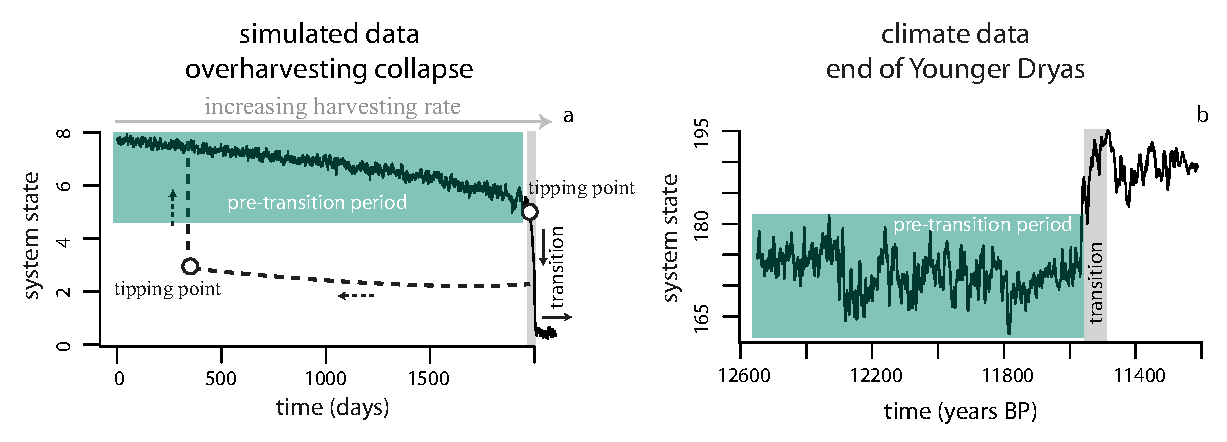
\includegraphics[scale=0.75]{figure_data.eps}
\caption{Datasets used: Simulated time series of resource biomass shifting to overexploitation (a), real-world time series of exit from Younger Dryas, the Earth's last climate shift from a cold period to the stable climate conditions as we know them today (b).}
\end{center}
%\label{fig:simulatedQDA}
\end{figure}

\section{Executables: Setting up the toolbox}
In order to execute the analyses proposed from our toolbox, two things are necessary:
1. to have access to internet,
2. to have R project for Statistical Computing installed on a computer,

R can be installed as it is freely available at \url{www.r-project.org/}. Instructions of how to install it on any operating system is fully documented. If you have R already installed, you need to make sure you are using a version (R>= 2.14.0). If needed, you can run an update of R.
Once you have installed R, start the program and, as shown in Fig. 2, copy-pasteon the command line:\\
\\
\textit{install.packages("devtools"); library(devtools); install\_github(repo = "earlywarnings-R", username = "earlywarningtoolbox", subdir = "earlywarnings")}\\
\\
Congratulations! You have just installed the Early Warning Signals Toolbox on your computer!

\begin{figure}[ht]
\begin{center}
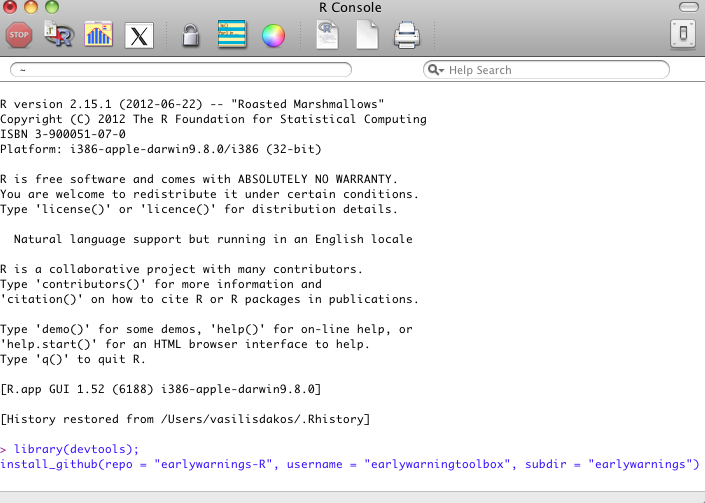
\includegraphics[scale=0.5]{R_install_ews.png}
\caption{Once R is installed, copy-paste the following lines in the console and press <enter>.}
\end{center}
%\label{fig:simulatedQDA}
\end{figure}

\section{Instructions: Using the toolbox}
What you want now to do is to get the user interface working to run the demo of the analysis presented in Part 1 of the submission. For this you need to copy-paste just one extra line:\\
\\
\textit{install.packages("shiny"); shiny::runGitHub("demo", "earlywarningtoolbox")}
\\

If everything has worked well, you should by now be in front of a window of your web-browser that should look like Fig. 3.
\newpage
\begin{figure}[ht]
\begin{center}
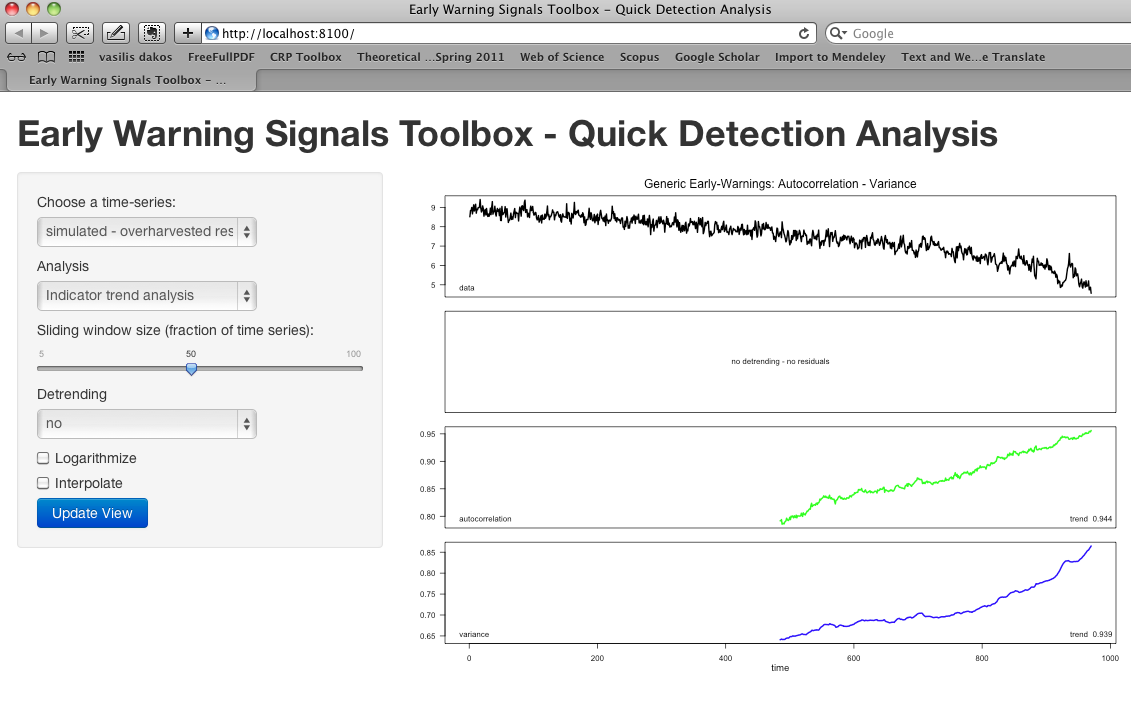
\includegraphics[scale=0.4]{demo_start.png}
\caption{User interface of the \textit{Indicator trend analysis} with Quick Detection.}
\end{center}
%\label{fig:simulatedQDA}
\end{figure}

You are ready to start using the Quick Detection Analysis! From the top drop-down method, you can choose the time series to use, \textit{simulated/ real-world data}, and from second top-down menu you can choose one of the three analysis that the Quick Detection offers: \textit{Indicator trend analysis, Trend significance analysis, Potential analysis}. After you choose an Analysis, different options appear. After any of your choices press Update View. Note that some calculations may take up some time, especially of the time series is long.
\\
\\
In case of the \textit{Indicator trend analysis} (Fig. 3), the options to select are:
\begin{enumerate}
\item \textit{Sliding window size} (the fraction along the time series to estimate variance and autocorrelation)
\item  \textit{Detrending} (filters data using smooth, linear, or first-difference detrending)
\item \textit{Logarithmize} (transforms the time series into logarithmic scale using \textit{log(x=1)})
\item \textit{Interpolate} (interpolates the time series in case there are missing values)
\end{enumerate}

\newpage
In case of the \textit{Trend significance analysis} (Fig. 4), the options to select are:
\begin{enumerate}
\item \textit{Sliding window size} (the fraction along the time series to estimate variance and autocorrelation)
\item  \textit{Detrending} (filters data using smooth, linear, or first-difference detrending)
\item \textit{Logarithmize} (transforms the time series into logarithmic scale using \textit{log(x=1)})
\item \textit{Interpolate} (interpolates the time series in case there are missing values)
\item \textit{Number of surrogate datasets} (to estimate a distribution of trends based from a null model without a transtion)
\item \textit{Level of significance} (to reject the null hypothesis)
\end{enumerate}

\begin{figure}[ht]
\begin{center}
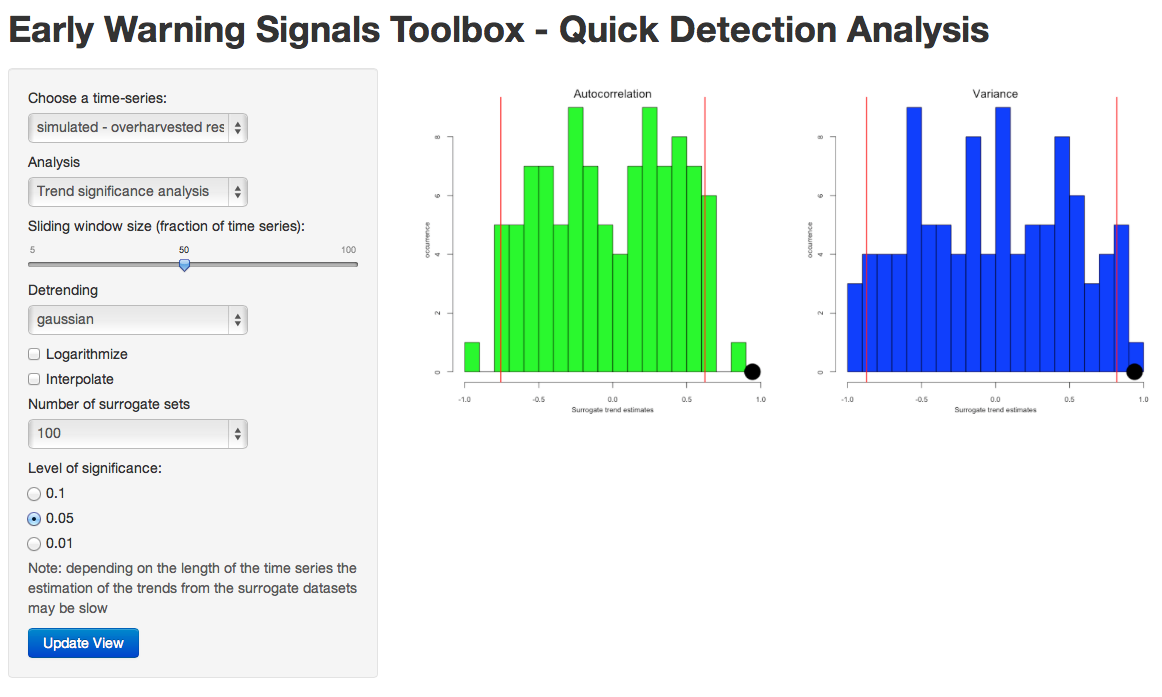
\includegraphics[scale=0.4]{demo_significance2.png}
\caption{User interface of the \textit{Trend significance analysis} with Quick Detection.}
\end{center}
%\label{fig:simulatedQDA}
\end{figure}
\newpage
In case of the \textit{Potential analysis} (Fig. 5), the options to select are:
\begin{enumerate}
\item \textit{Threshold} (for detecting local minima ~ alternative attractors)
\item \textit{Grid size} (for determining the analysis resolution)
\item \textit{Cutoff level} (to clarify the visualization)
\end{enumerate}

\begin{figure}[ht]
\begin{center}
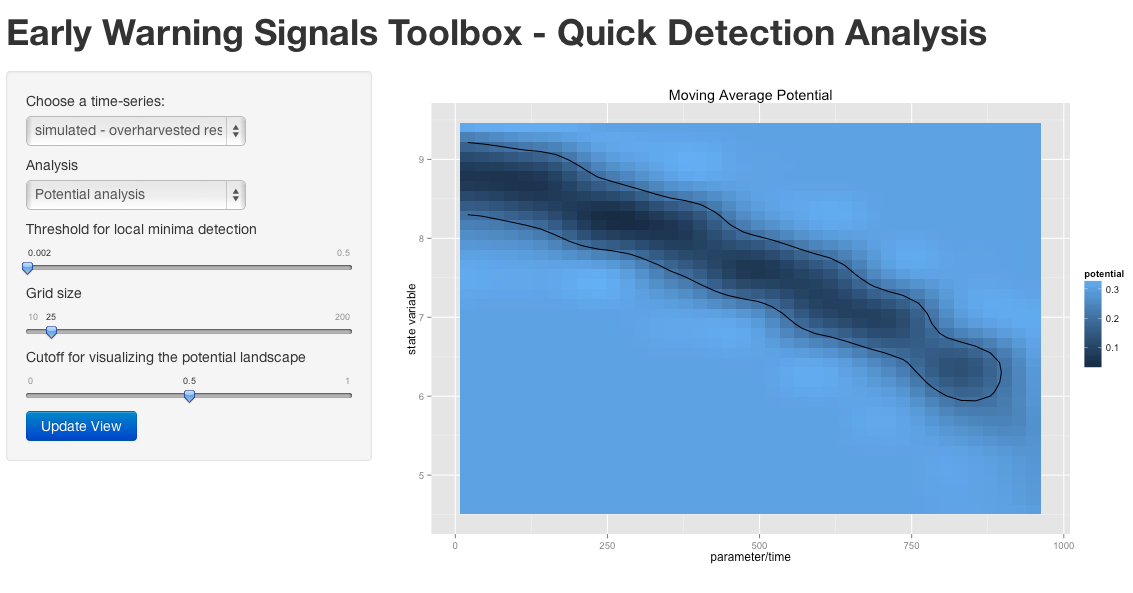
\includegraphics[scale=0.4]{demo_potential.png}
\caption{\textit{Potential Analysis} with Quick Detection.}
\end{center}
%\label{fig:simulatedQDA}
\end{figure}

\end{doublespacing}


\end{document}

